\documentclass[a4paper,12pt]{article}
\usepackage[a4paper,top=1.3cm,bottom=2cm,left=1.5cm,right=1.5cm,marginparwidth=0.75cm]{geometry}
\usepackage{cmap}
\usepackage{mathtext}
\usepackage[T2A]{fontenc}
\usepackage[utf8]{inputenc}
\usepackage[english,russian]{babel}
\usepackage{siunitx}

\usepackage{graphicx}

\usepackage{wrapfig}
\usepackage{tabularx}
\usepackage{multirow}

\usepackage{hyperref}
\usepackage[rgb]{xcolor}
\hypersetup{
colorlinks=true,urlcolor=blue
}
\usepackage{amsmath,amsfonts,amssymb,amsthm,mathtools}
\usepackage{icomma}
\mathtoolsset{showonlyrefs=false}
\usepackage{euscript}
\usepackage{mathrsfs}
\DeclareMathOperator{\sgn}{\mathop{sgn}}
\newcommand*{\hm}[1]{#1\nobreak\discretionary{}
{\hbox{$\mathsurround=0pt #1$}}{}}

%%% Заголовок
\author{Макаров Лев Евгеньевич}
\title{Лабораторная работа №3.4.2

Закон Кюри-Вейсса
}
\date{\today}

\begin{document}

\begin{titlepage}
	\begin{center}
		{\large МОСКОВСКИЙ ФИЗИКО-ТЕХНИЧЕСКИЙ ИНСТИТУТ (НАЦИОНАЛЬНЫЙ ИССЛЕДОВАТЕЛЬСКИЙ УНИВЕРСИТЕТ)}
	\end{center}
	\begin{center}
		{\large Физтех-школа фотоники, электроники и молекулярной физики}
	\end{center}
	
	
	\vspace{4.5cm}
	{\huge
		\begin{center}
			{\bf Отчёт о выполнении лабораторной работы 3.4.2}\\
			Закон Кюри-Вейсса
		\end{center}
	}
	\vspace{2cm}
	\begin{flushright}
		{\LARGE Автор:\\ Макаров Лев Евгеньевич \\
			\vspace{0.2cm}
			Б04-306}
	\end{flushright}
	\vspace{8cm}
	\begin{center}
		Долгопрудный 2024
	\end{center}
\end{titlepage}

\section{Введение}

\textbf{Цель работы:} 
\begin{enumerate}
	\item изучение температурной зависимости магнитной восприимчивости ферромагнетика выше точки Кюри
\end{enumerate}

\textbf{В работе используются:} 
\begin{itemize}
    \item катушка самоиндукции с образцом из гадолиния
    \item термостат
    \item частотомер
    \item цифровой вольтметр
    \item LC-автогенератор
    \item термопара медь–константан
\end{itemize}
\medskip

\section{Теоретические сведения}

В данной лабораторной работе предлагается проверить закон Кюри-Вейсса: при температуре выше температуры Кюри:

\begin{equation*}
    \chi \sim \frac{1}{T - \theta_P}
\end{equation*}

$\theta_P$ - парамагнитная точка Кюри.

Исследуемый материал будет помещен в катушку индуктивности, из-за чего её индуктивность будет меняться с температурой:

\begin{equation*}
    L - L_0 \sim \mu - 1 = \chi
\end{equation*}

Изменение индуктивности будем наблюдать с помощью изменения периода колебаний: $\tau = 2\pi\sqrt{LC}$, поэтому 

\begin{equation*}
    L - L_0 \sim \tau^2 - \tau_0^2 \ \rightarrow \ \chi \sim \tau^2 - \tau_0^2 \ \ \rightarrow \ \frac{1}{\tau^2 - \tau_0^2} \sim T - \theta_P
\end{equation*}

Здесь $L_0$ и $\tau_0$ - индуктивность и период колебаний без образца в катушке соответственно.

\section{Эксперементальная установка}

Исследуемый ферромагнитный образец (гадолиний) расположен внутри пустотелой катушки самоиндукции, которая служит индуктивностью колебательного контура, входящего в состав $L C$ -автогенератора.

\begin{center}
    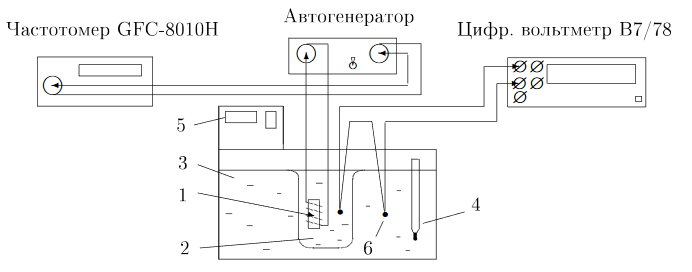
\includegraphics[width=0.8\textwidth]{ustan.png}
    \label{pic:1}
\end{center}

Катушка 1 с образцом помещена в стеклянный сосуд 2, залитый трансформаторным маслом. Масло предохраняет образец от окисления и способствует ухудшению электрического контакта между отдельными частичками образца. Кроме того, оно улучшает тепловой контакт между образцом и рабочей жидкостью 3 в термостате. Ртутный термометр 4 используется для приближённой оценки температуры.

При изменении температуры меняется магнитная восприимчивость образца $\chi,$ а следовательно, самоиндукция катушки и период колебаний $\tau$ автогенератора. Для измерения периода используется частотомер.

Измерения проводятся в интервале температур от $14^{\circ} \mathrm{C}$ до $40^{\circ} \mathrm{C}.$ 

Температура исследуемого образца всегда несколько отличается от температуры дистиллированной воды в сосуде. Эта разность температур фиксируется термопарой, чувствительность которой $\mathrm{K}=24\frac{\text{град}}{\text{мВ}}$. ЭДС термопары измеряется цифровым вольтметром.

\section{Результаты измерений и обработка данных}

\subsection{подготовка приборов}

Включим все приборы и выберем необходимые режимы измерения. Включим термостат и выставим нужную температуру.

\subsection{Оценка ЭДС}

В работе допустимая разность температур образца и воды в термостате $\Delta T = 0,5 \ C^\circ$. Температурный коэффициент термопары $K = 24 \text{град}/\text{мВ}$. Тогда допустимая ЭДС:

\begin{equation*}
    \Delta U = 0,02 \ \text{В}
\end{equation*}

\subsection{Зависимость периода от температуры}

Измерим зависимость периода колебаний от температуры образца. Будем выставлять температуру термостата и ждать пока ЭДС не будет меньше $\Delta U$. После чего измерять период при этой температуре. Результаты запишем в таблицу \ref{table:1}.

\begin{table}[!ht]
    \centering
    \begin{tabular}{|l|l|l|l|}
    \hline
        $N$ & $t$, $C^\circ$ & $U$, мВ & $\tau$, мкс \\ \hline
        1 & 14,02 & -0,011 & 10,7929 \\ \hline
        2 & 16,01 & -0,019 & 10,693 \\ \hline
        3 & 18,04 & -0,016 & 10,528 \\ \hline
        4 & 20,07 & -0,0154 & 10,21502 \\ \hline
        5 & 22,05 & -0,018 & 9,878 \\ \hline
        6 & 24,01 & -0,132 & 9,545 \\ \hline
        7 & 26,01 & -0,147 & 9,4184 \\ \hline
        8 & 28,07 & -0,0182 & 9,34852 \\ \hline
        9 & 30,06 & -0,0178 & 9,3002 \\ \hline
        10 & 32,05 & -0,0184 & 9,267 \\ \hline
        11 & 34,03 & -0,0185 & 9,244 \\ \hline
        12 & 36,03 & -0,0155 & 9,2253 \\ \hline
        13 & 38,02 & -0,0158 & 9,21023 \\ \hline
        14 & 40,00 & -0,0169 & 9,198824 \\ \hline
    \end{tabular}\caption{\textit{Зависимость периода колебаний от температуры}}\label{table:1}
\end{table}

Здесь: $\sigma_\tau = 0,003$ мкс, а $\sigma_T = 0,03, C^\circ$

\subsection{Период без образца}

Период колебаний без образца:

\begin{equation*}
    \tau_0 = (9,045 \pm 0,003) \ \text{мкс}
\end{equation*}

\subsection{Завершение измерений}

После измерений отключим термостат и все приборы.

\subsection{Определение парамагнитной точки Кюри}

Используя показания термопары, вычислим температуру образца. Все вычисления запишем в таблицу \ref{table:2}.

\begin{table}[!ht]
    \centering
    \begin{tabular}{|l|l|l|c|}
    \hline
        $N$ & $t$, $C^\circ$ & $T$, К & $1/(\tau^2 - \tau_0^2)$, $\text{мкс}^{-2}$ \\ \hline
        1 & 14,02 & 286,8 & 0,0288 \\ \hline
        2 & 16,01 & 288,6 & 0,0307 \\ \hline
        3 & 18,04 & 290,7 & 0,0345 \\ \hline
        4 & 20,07 & 292,7 & 0,0444 \\ \hline
        5 & 22,05 & 294,6 & 0,0634 \\ \hline
        6 & 24,01 & 293,8 & 0,1076 \\ \hline
        7 & 26,01 & 295,5 & 0,1450 \\ \hline
        8 & 28,07 & 300,6 & 0,1791 \\ \hline
        9 & 30,06 & 302,6 & 0,2136 \\ \hline
        10 & 32,05 & 304,6 & 0,2460 \\ \hline
        11 & 34,03 & 306,6 & 0,2748 \\ \hline
        12 & 36,03 & 308,7 & 0,3036 \\ \hline
        13 & 38,02 & 310,6 & 0,3315 \\ \hline
        14 & 40,00 & 312,6 & 0,3563 \\ \hline
    \end{tabular}\caption{\textit{Зависимость периода колебаний от температуры}}\label{table:1}
\end{table}

Построим график зависимости $1/(\tau^2 - \tau_0^2) = f(T)$. Для построения графика используем точки, лежащие на прямой. График изобразим на рисунке \ref{graph:1}.

\begin{figure}[!ht]
        \centering
	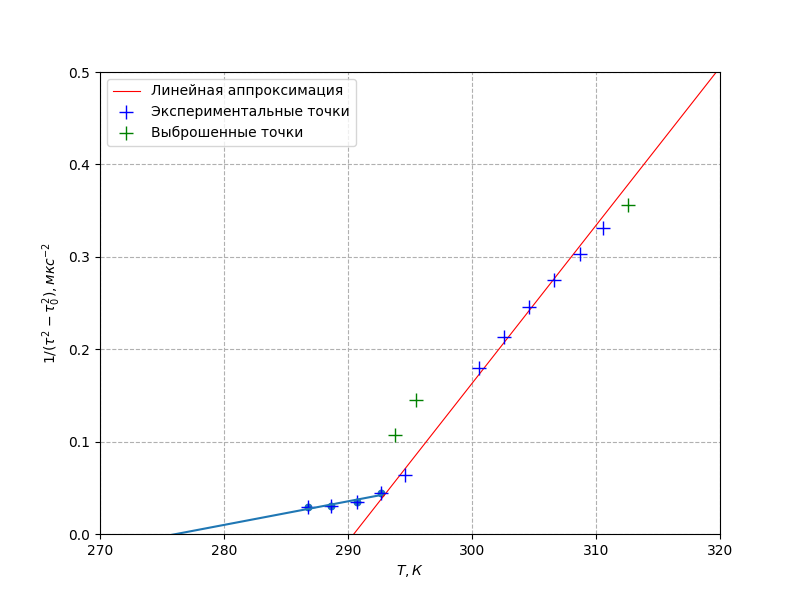
\includegraphics[width=1.0\textwidth]{tau_t.png}
	\caption{\textit{Зависимость силы от квадрата индукции для всех измерений}}
	\label{graph:1}
\end{figure}

Часть точек было решено выбросить, так как они явно вносят большую ошибку.

Параметры полученной прямой:

\begin{equation*}
    k = (0,0171 \pm 0,0005) \ \text{К}^{-1} \cdot \text{мкс}^{-2} \ \ \ \ \ b = (-4,968 \pm 0,002) \ \text{мкс}^{-2}
\end{equation*}

Теперь находим точку Кюри:

\begin{equation*}
    \theta_p = - \frac{b}{k} = (290 \pm 9) \ \text{К}
\end{equation*}

\subsection{Определение ферромагнитной точки Кюри}

Часть точек не лежащую на прямой аппроксимируем экспонентой. Тогда температура Кюри:

\begin{equation*}
    \theta_K = (276 \pm 9) \ \text{К}
\end{equation*}

\subsection{Сравнение результатов}

Полученные значения в пределах погрешности совпали с табличными.

\end{document}